\cut{
\begin{itemize}
\item Compiler
  \begin{itemize}
  \item Camlp4, tcc, and fmlc (generate typedefs and prefeed defs) 
  \end{itemize}

\item Runtime system
  \begin{itemize}
  \item data structure of feed items: iData, meta data, etc
  \item implementation of feed/stream: lazy list
  \item fetching mechanism: eager fetching vs. lazy consumption, 
    http\_client library, batch fetching
  \item parse using padsML easy lib
  \item concurrency
  \item error handling
  \item discussion of selected combinators: local pairing, 
    dependent pairing (separate thread/queue)
  \end{itemize}

\item Tools library
  \begin{itemize}
  \item use of generic tool framework and feeds runtime lib
  \item use of several external ocaml libs: rrdtools, xml\_light
  \end{itemize}

\item Future work (shall we include???)
  \begin{itemize}
  \item expose meta data to the surface language
  \item a second (simplified) prefeed def with type defs only
  \end{itemize}

\item Experiments
  \begin{itemize}
  \item performance metrics: throughput, network/system latency
  \item setup (mac powerbook g4, 100Mb ethernet connection, 
    comon spec, comon nodes, random selection of nodes)
  \item two tables and graphs: throughput peaks at 
    200 nodes (chunk size), sys latency almost constant,
    system is scalable to comon (842 nodes)
  \end{itemize}
\end{itemize}
}

The \padsd{} implementation has three parts: the compiler, the runtime
system, and the built-in tools library. We describe these
parts in turn and then evaluate the overall system performance and design.

%%In this section, we describe
%%these parts and evaluate the performance of the system. We conclude
%%with a discussion of our choice to design a language
%%extension to \ocaml{} as opposed to providing a library.
%We will show that the system can easily scale
%to support PlanetLab-sized applications with 
%hundreds of nodes. 

\paragraph*{The Compiler.}
The \padsd{} compiler consists of
\cd{tcc}, the tool configuration compiler for .tc files, 
and 
\cd{fmlc}, the compiler for feed declarations (.fml files). 
Both compilers convert their sources into \ocaml{} code, which is then
compiled
and linked to the runtime libraries.  We implemented both tools with
\camlp{}, the \ocaml{} preprocessor. 

% \begin{figure}[t]
% \centering
% \begin{codebox}
% let simple_comon =
% \{\kw{frep} = fun ff ->
%  ff.\kw{all}
%  \{Combinators.\kw{format} = Comon_format.Source.parse;
%   \kw{print} = Comon_format.Source.print;
%   \kw{format_rep} = Comon_format.Source.tyrep; 
%   \kw{incremental} = false;
%   \kw{header_format} = None; 
%   \kw{locations} = sites;
%   \kw{schedule} =
%     Schedule.{\kw every} (Time.now (), 10., 
%                     Schedule.default_duration, 60.);
%   \kw{has_records} = Comon_format.__PML__has_records; 
%   \kw{pp} = None\}\}
% \end{codebox}
% \caption{Code fragment of compiled simple\_comon feed}\label{fig:compiledcomon}
% \end{figure}

%A source program is parsed into an abstract
%syntax tree defined by the Camlp4 extended syntax, and the
%code generation is done through the quotation system. 
The \cd{fmlc} compiler performs code generation in two steps.
First, the code generator emits the
type declarations for each feed.  
%% FIXME: is what is meant by representations clear here? (ksf)
Second, it generates representations for each feed description.  
The compiler constructs these representations
by extracting elements from the concurrently
generated \padsml{} libraries
and using polymorphic combinators to build structured 
descriptions.  
%Figure \ref{fig:compiledcomon} shows a fragment of
%the compiled code for
%the simple CoMon feed in Figure \ref{fig:simplecomon}.
%%While a programmer could use our combinator library directly, the
%%surface syntax provides a simple veneer that reduces the barrier to
%%entry substantially.
% in a
%lazy fashion (that is, only generate the declaration if the
%feed is used in the rest of the description).
%In the second step, 
%,
%also known as the ``prefeed''. Schedules which are
%definite times such as ``2008/09/30:12:00:00'' or ``5 mins'' are
%converted to floating point number of seconds at compile time
%to make the code more efficient.
%All O'Caml expressions embedded in the fml file are
%included without change in the compiled code. 

\paragraph*{The Runtime System.}
We implement each \padsd{} feed as a lazy list of feed items. 
Following the semantics in \secref{sec:semantics}, 
a feed item is a (meta-data, payload) pair, 
although the implementation has a more refined notion of meta-data
that includes more detailed error information.
% for HTTP errors, late item arrivals, parse errors, \etc{}

% Late arrival, (3)
% %{{\small{ 
% \begin{verbatim}
% 1: Misc HTTP error
% 2: Late arrival
% 3: Ssh host required
% 4: Remote command required for ssh
% 5: Bad message
% \end{verbatim}
% %}}} \normalsize

% % This means the feed 
% % is actually a function {\tt next}. It is evaluated 
% % only when the user program attempts to take an
% % item from the feed. The function {\tt next} returns an
% % item plus a new {\tt next} function which represents
% % the tail of the feed.
% %a data item of polymorphic type 'a and 
% %a meta data structure that corresponds 'a. 
% %The type of a feed is also the type of its data item. 
% %The type of a base feed has an option type.
% The meta data is a tree structure in which
% each node is tagged with a meta header. 
% The tree structure (also known as the meta body) resembles 
% the structure of the data item, i.e.  if the data item is a pair, 
% then the meta body is also a pair of meta data. Each leaf
% of the meta body corresponds to a base feed. Meta information
% such as the scheduled time, arrival time, location and 
% errors is stored in the leaves. The header records the summary 
% of meta information within the subtree. 

The \padsd{} runtime system is a multi-threaded concurrent
system that follows the  master-worker implementation strategy. 
%Each base feed is created and maintained by a separate 
%worker thread, and a master thread drives the combination of 
%base feeds into compound feeds.  
Each worker thread either fetches data from a specified
location and parses the data into an internal representation (the {\em rep}),
%(known as the {\em rep})
or synthesizes its data by calling a
generator function.  Using error conditions, location, scheduled time
and arrival time, the worker generates the appropriate meta-data,
pairs it with the rep and pushes the feed item onto a queue. 
%And then it generates the idata from the rep and the meta data,
%and pushes the idata into the concurrent queue.
%The workers communicated with
%the master through a concurrent queue.
The master thread pops the feed item from the queue on demand, \ie{},
when the user program requests the data. 
The worker thread is {\em eager}, which guarantees that all 
data will be fetched and archived, but the master thread is 
{\em lazy}, which allows application programs to process only relevant
data. 

%The concurrency control is implemented by the O'Caml threads
%library using standard mutex and condition variables.

We used the \ocamlnet{} library~\cite{ocamlnet2} to implement
the fetching engine. It batches concurrent fetch requests into groups
of 200, a size which balances maximizing throughput with avoiding
overwhelming the operating system with too many open sockets.


%Given a list of locations to fetch from at any one time, 
%the system converts the list into batches and fetches up to 200 locations
%per batch. The choice of 200 is a trade-off between maximizing
%the throughput and avoiding overwhelming the operating system
%with too many open sockets. 
%If the system fails to fetch an
%item due to network or system error, a feed item is still created
%with the appropriate error code written in the meta-data. 

% The \padsd{} system does not 
% automatically filter out erroneous items because errors often 
% provides very important information to users who monitors 
% distributed systems. Users could optional choose to filter
% out bad feed items using the Feed library functions.

% Compound feeds are created within the generic tool framework by
% combining base feeds using various combinator functions.
% These functions takes idatas from two feeds and creates a new idata often
% by comparing the timestamps in the two idatas. While this is done
% lazily in most of the combinators, it is not the case for
% dependent pairs. This is because the dependent feed needs to be
% created {\em eagerly} when each item from the {\em depending}
% feed arrives. Therefore we add another layer of ``pseudo-fetching"
% for the dependent feed. Here a separate thread is created for each
% dependent feed, which actively takes data from the depending
% feed, creates dependent items, and push to another concurrent
% queue of its own.  
 
\paragraph*{Tools Library.}
As explained in Section~\ref{sec:programming}, we implemented the
\padsd{} off-the-shelf tool suite using our generic tool framework. 
%Many of the tools rely upon format-specific libraries generated 
%from format specifications.
Some tools depend upon auxiliary tools.  
For instance, the feed selector calls a data selector built using
the \padsml{} generic tool framework \cite{padsml-padl} for base feeds.
%For instance, the
%feed selector relies upon a data selector generated by type-directed
%compilation of the \padsml{} description.
Other tools depend upon external libraries. For instance, the
\cd{feed2rrd} tool requires the RRD round-robin database~\cite{rrdtool} and
the \cd{feed2rss} tool uses the XML-Light package~\cite{xmllight} for
parsing and printing XML.
%The system also provides an Feed interface to a number of
%useful runtime functions such as map and fold for advanced
%users to program against the feeds.

\cut{
\begin{table*}[th]
\begin{center}
\begin{tabular}{|l|r|r|r|r|r|r|r|r|r|r|r|r|}\hline
Num of nodes&	50&	100&	150&	200&	250&	300&	350&	400&	450&	500&	550&	600 \\ \hline\hline
Net latency per node (secs)&	9&	4&	4&	4&	8.6&	5.3&	19.1&	19.5&	14.4&	7.8&	12&	13.3 \\ \hline
Sys latency per node (secs)&	0&	0&	0&	0.3&	0.2&	0.4&	0.3&	0.1&	0.3&	0.4&	0.2&	0.7 \\ \hline
%Total Latency (secs)&	9&	4.04&	4&	4.3&	8.8&	5.8&	19.4&	19.6&	14.7&	8.2&	12.3&	14 \\ \hline
Total fetch time (secs)&	9&	5&	4&	5&	23&	9&	22&	23&	26&	14&	27&	28 \\ \hline	
Throughput (items/sec)&	5.6&	20&	37.5&	40&	10.9&	33.3&	15.9&	17.4&	17.3&	35.7&	20.4&	21.4 \\ \hline
\end{tabular}
\end{center}
\caption{Performance of CoMon without archiving}
\label{tab:comon-noarch}
\end{table*}


\begin{table*}
\begin{center}
\begin{tabular}{|l|r|r|r|r|r|r|r|r|r|r|r|r|}\hline
Num of nodes&	50&	100&	150&	200&	250&	300&	350&	400&	450&	500&	550&	600 \\ \hline\hline
Net latency per node (secs)&	16&	4&	4&	4&	18.9&	6&	20.6&	22&	8.4&	13&	21.8&	21.3 \\ \hline
Sys latency per node (secs)&	0.8&	1.28&	1.4&	1.8&	1.9&	1.5&	1.6&	1.3&	1.9&	1.7&	1.7&	2.2 \\ \hline
%Total Latency (secs)&	16.8&	5.28&	5.4&	5.8&	20.8&	7.5&	22.2&	23.3&	10.3&	14.7&	23.56&	23.5 \\ \hline
Total fetch time (secs)&	17&	6&	7&	7&	27&	12&	27&	30&	19&	33&	43&	43 \\ \hline
Throughput (items/sec)&	2.9&	16.7&	21.4&	28.6&	9.3&	25&	13&	13.3&	23.7&	15.2&	12.8&	14 \\ \hline
\end{tabular}
\end{center}
\caption{Performance of CoMon with archiving}
\label{tab:comon-arch}
\end{table*}
}

\paragraph*{Experiments.} \label{sec:experiments}

\begin{figure}[t]
\begin{center}
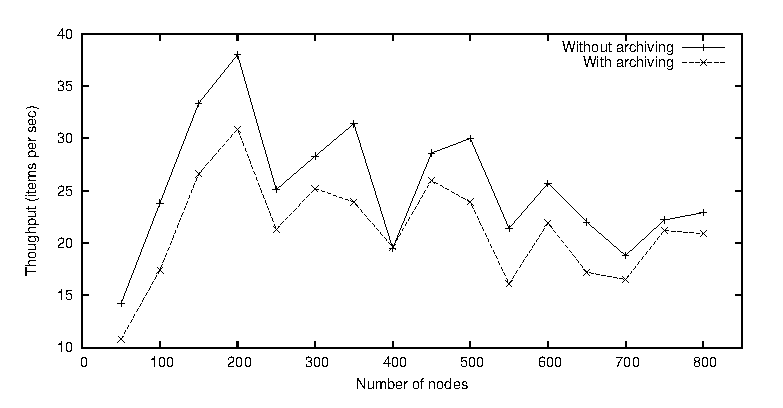
\epsfig{file=throughput.eps, width=\columnwidth}
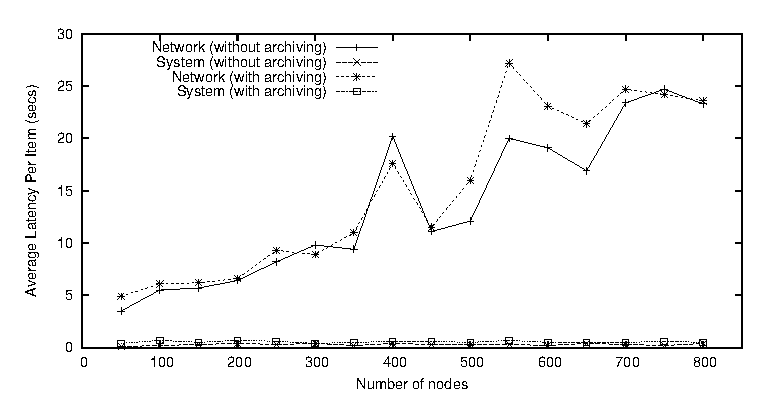
\epsfig{file=latency.eps, width=\columnwidth}
\caption{Average throughput and latencies per node}
\label{fig:throughput}
\end{center}
\end{figure}

To assess performance, we measure 
the average time to fetch a data item (termed {\em network latency}), 
the average time to prepare the data item for consumption
after fetching it from the network (termed {\em system latency}),
and the {\em throughput} of the system for the CoMon feed
description in \figref{fig:feedcomon}. 
The throughput measures the average
number of items fetched and processed per second. 
%We picked
%the comon example because it is a real life
%application that involves fetching from large number of 
%nodes (800+) at the same time, which can be viewed as a stress test. 

All the experiments were conducted on a Mac Powerbook G4 computer
with a 1.67GHz CPU and 2GB memory running Mac OS X 10.4.
%connected to the Internet via 11Mb/s wireless ethernet.
In each experiment, we randomly selected 16 subsets of PlanetLab
nodes, with increasing size from 50 to 800 in increments of 50.
%%In each experiment, we randomly selected 50 nodes,
%%100 nodes, up to 800 PlanetLab nodes
%\footnote{List taken from http://www.cs.princeton.edu/~vivek/node\_list\_all. 
%Nodes could come and go sporadically.} 
%%to form 16 node sets. 
For each set, we applied the profiler tool for the CoMon feed
twice, once without archiving and once with it, to measure the
throughput and latencies as the system fetched from these node lists. 
We repeated the experiment ten times and calculated the average values.

\figref{fig:throughput} shows the average throughput
and the average network and system latencies.
The throughput is maximized when fetching from 200 nodes because
the system supports up to 200 concurrent fetches.
%Generally, 
%the throughput goes up with the number of nodes
%until 200 and then starts declining and saturating
%as it approaches 800. Locally, 
%the throughput hits peaks at multiples of 200 since the system supports 
%up to 200 concurrent fetches.
%is the size of the
%fetching batch. At multiples of 200, the concurrent
%fetching is maximally utilized. 
%An anomaly occurred at 400 nodes, as a number of nodes were unreachable
%because of DNS failures.
% at the time of
%the experiment. 
Archiving adds to the overhead of the system and hence
reduces the throughput and increases network and system latencies. 
Note that while network latency increases with the number of nodes,  
system latency remains almost constant and relatively
low, showing that the \padsd{} runtime system adds
little overhead to the inevitable network fetching
cost. Despite the random network delays in these experiments,
the network latency is generally linear in the number of nodes. 
The system, which we have not tried to optimize, was able to fetch
data from 
800~nodes and archive the results in under 70~seconds, well under the
5 minute turnaround time currently supported by CoMon. 
Taken together, these results suggest that \padsd{} is
capable of supporting PlanetLab-scale monitoring. 

%Tables \ref{tab:comon-noarch} and \ref{tab:comon-arch}
%shows the results from two different scenarios:
%one in which the user program simply creates the comon feed without applying
%any tools on it, and one in which the comon feed is created
%and archived. In both scenarios, the system was
%able to fetch from up to 600 nodes within one minute, which is
%significantly shorter than the 5-minute turnaround time in the real
%CoMon system.
%\begin{figure}[th]
%\begin{center}
%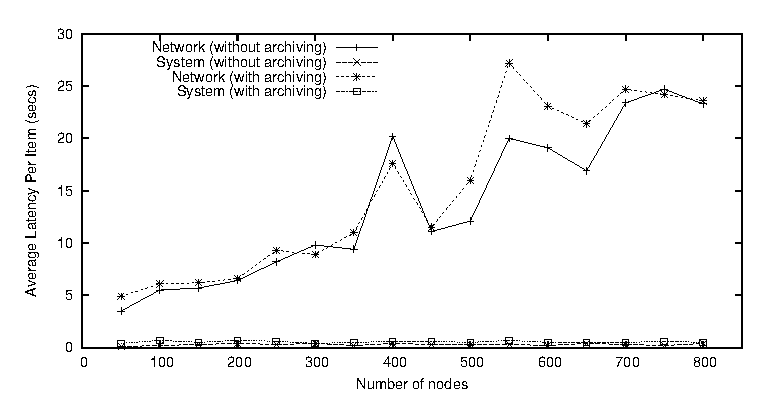
\epsfig{file=latency.eps, width=\columnwidth}
%\caption{Average latencies per node}
%\label{fig:latency}
%\end{center}
%\end{figure}

\cut{
We plot the average throughput in Figure \ref{fig:throughput}
and the system and network latencies in Figure \ref{fig:latency}. 
As expected, both the throughput and latency suffer a little with 
archiving taking place. The throughput peaks when fetching from
200 nodes because 200 is the size of the fetching batch and
at 200 nodes, the concurrent fetching engine is maximally utilized.
The experiment for 450 nodes exhibits an anomaly as the archived
experiment takes less time than the un-archived experiment.
This is probably due to sudden delays in some of the nodes when the
no-archiving experiment is run. One obvious take-away from
Figure \ref{fig:latency} is that while the network latency may
vary greatly depending on the network condition, the system latency
stays almost constant at relatively low levels. This shows that
the \padsd{} system runtime adds little overhead to the 
inevitable network cost, which means the system could scale to
large applications. 
}

\paragraph*{Language or Library.}
There is the natural question of whether the system is better
implemented as a library than a language extension. We chose
to present our work as a language because: (1) the compiler automatically
eliminates boilerplate code; (2) the surface syntax simplifies the coding of
the underlying higher-order interfaces; and (3) a language approach allows
smooth integration with \padsml which itself is a successful 
language extension.


\cut{%%%%%%%%%%%%%%%%%%

\subsection{Language or Library}
% reason (4) managing functors & modules?
Our feed language is a veneer on \ocaml{} built with the \camlp{}
preprocessor.   
A natural question is whether the system would be better
implemented as a library rather than a language extension.  For the reasons
described in the following paragraphs, we chose to present our work as a
language. 

\textbf{\textit{Automatic elimination of boilerplate code.}}
The compiler eliminates boilerplate code by
(a) generating both type declarations and values from 
descriptions (particularly record types and datatypes), something
that cannot be done in a library, (b) packaging definitions
in modules for name-space management and functor usage, 
(c) automatically filling in defaults for values omitted from
configuration files, and (d) generating complete, stand-alone executables from
declarative descriptions and configurations. 
%Much of the boilerplate 
%elimination is achieved by parsing fml and config files, filling in 
%defaults and automatically generating driver programs for the naive 
%user that string together generic tools.  Other boilerplate is avoided
%by generating both types and values automatically from descriptions
%(particularly datatype descriptions) and packaging them inside modules.

\textbf{\textit{Syntax and simplicity of coding style.}}  The underlying
interfaces are {\em very} higher-order, which, without surface sugar,
would force a complex coding style on the off-the-shelf user.
For instance, almost every line of a description would be translated
to an increasingly nested combinator application, and every variable binding
would induce a use of higher-order abstract syntax. 

\textbf{\textit{Generic programming.}} \ocaml{} (and most other 
potential host languages)
has no direct support for
the generic programming needed to implement the tool suite.  After considerable
study, the most effective way we have found to provide the required 
generic programming interface involves judicious use of unsafe casts
under the covers.  By generating type representations using the compiler,
we guarantee these casts cannot go wrong.

% \textbf{\textit{Compile-time schedule analysis.}} The synchronous
% pair and list feed comprehension combinators are intended for subfeeds
% that share the same schedule.  Using them otherwise is likely an error.
% We anticipate future work on schedule analysis to detect such errors 
% and to help us optimize our implementation.  
% %Such analysis is easier in language framework.  


\textbf{\textit{Integration with \pads{}.}}  Core
\pads{}~\cite{fisher+:pads,fisher+:popl06,fisher+:dirttoshovels,mandelbaum+:pads-ml} has had success as a language extension on top of C as well as
\ocaml{}.  Its purpose is to describe and document properties of ad hoc
data sources as well as to facilitate generation of local, single-source 
tools.  Extending such descriptions to include source location, 
availability and 
access mode helps complete the documentation in a single centralized 
specification and through a uniform notation.  It gives off-the-shelf
users everything they need in a single language.  Forcing a division 
of the specification into part library/part language would ruin its
cohesiveness, particularly in the context of
dependent feeds where there is tight interplay between access mode, location,
schedule and format.


%Having made our case for a language extension, the bulk of our implementation
%{\em is} a collection of libraries.  Hence, the intrepid hacker may eschew our
%surface syntax and program directly against the interfaces underneath.
%Whatever the programmer chooses, the central contribution of this work
%are the abstractions we provide.  Moreover
Though we believe our current design is well motivated,
we also believe the ideas presented here can transcend
their current implementation.  By defining a compact feed calculus 
with a precise semantics, we allow the possibility for
others to embed our abstractions directly in a language
such as Haskell that provides superior support for generic programming. 
%%and the ability to avoid boilerplate by automatically deriving 
%%implementations from type classes.

}%%%%%%%%%%%%%%%%%%%%
